\documentclass[11pt]{article}
\usepackage[margin=1in]{geometry}
\usepackage{graphicx}
\usepackage{float}
\usepackage{booktabs}
\usepackage{siunitx}
\usepackage{amsmath}
\usepackage{amssymb}
\usepackage{pgfplots}
\usepackage{pgfplotstable} % Added for dynamic table import
\usepackage{subcaption}
\usepackage{listings}
\usepackage{xcolor}

\pgfplotsset{compat=1.18}

% Code listing style configuration
\definecolor{codegreen}{rgb}{0,0.6,0}
\definecolor{codegray}{rgb}{0.5,0.5,0.5}
\definecolor{codepurple}{rgb}{0.58,0,0.82}
\definecolor{backcolour}{rgb}{0.95,0.95,0.92}

\lstdefinestyle{mystyle}{
  backgroundcolor=\color{backcolour},
  commentstyle=\color{codegreen},
  keywordstyle=\color{magenta},
  numberstyle=\tiny\color{codegray},
  stringstyle=\color{codepurple},
  basicstyle=\ttfamily\footnotesize,
  breakatwhitespace=false,
  breaklines=true,
  captionpos=b,
  keepspaces=true,
  numbers=left,
  numbersep=5pt,
  showspaces=false,
  showstringspaces=false,
  showtabs=false,
  tabsize=2
}
\lstset{style=mystyle}

\title{\textbf{ENGR 200: Lab 5}\\
Data Acquisition, Digitization, and Sampling}
\author{Sean Balbale}
\date{March 2026}
\setlength{\parindent}{0in}
\setlength{\parskip}{\baselineskip}

\begin{document}

\begin{titlepage}
  \begin{center}
    \vspace*{1in}

    \Huge
    \textbf{Lab 5}

    \LARGE
    Data Acquisition, Digitization, and Sampling

    \vspace{3in}

    \textbf{Student Name:} Sean Balbale
    \\ \textbf{Course:} Engineering 200
    \\ \textbf{Instructor:} Prof. R. Gao
    \\ \textbf{Date:} March 2026

    \vfill

  \end{center}
\end{titlepage}

\newpage

% ---------------------------------------------------------
% PART 1: ALIASING
% ---------------------------------------------------------
\section*{Part 1: The Effects of Undersampling (Aliasing)}

In this task, a \SI{5.0}{\volt} peak-to-peak sine wave was sampled at a constant rate of $f_s = \SI{2000}{\hertz}$ while the true signal frequency was swept from \SI{500}{\hertz} to \SI{2500}{\hertz} in \SI{100}{\hertz} increments. The Nyquist frequency for this system is exactly \SI{1000}{\hertz} ($f_s / 2$).

\begin{table}[H]
  \centering
  \caption{Complete Theoretical Alias Frequency Predictions ($f_s = 2000$ Hz)}

  % Dynamically import the text file and format it as a table
  \pgfplotstabletypeset[
    header=false,        % Tells LaTeX not to use the txt file's header
    skip first n=1,      % Skips the first line of the txt file to avoid space-parsing errors
    columns={0, 1, 2, 3}, % Grab the 4 data columns
    display columns/0/.style={column name={\textbf{Function Freq (Hz)}}},
    display columns/1/.style={column name={\textbf{Sampling Freq (Hz)}}},
    display columns/2/.style={column name={\textbf{Nyquist Freq (Hz)}}},
    display columns/3/.style={column name={\textbf{Alias Freq (Hz)}}},
    every head row/.style={before row=\toprule, after row=\midrule}, % Adds top/mid lines
    every last row/.style={after row=\bottomrule},                   % Adds bottom line
    col sep=space        % Tells LaTeX the data is separated by spaces
  ]{../Task1_Alias_Table.txt} % Path to your text file

\end{table}

\begin{figure}[H]
  \centering
  \begin{subfigure}{0.48\textwidth}
    \centering
    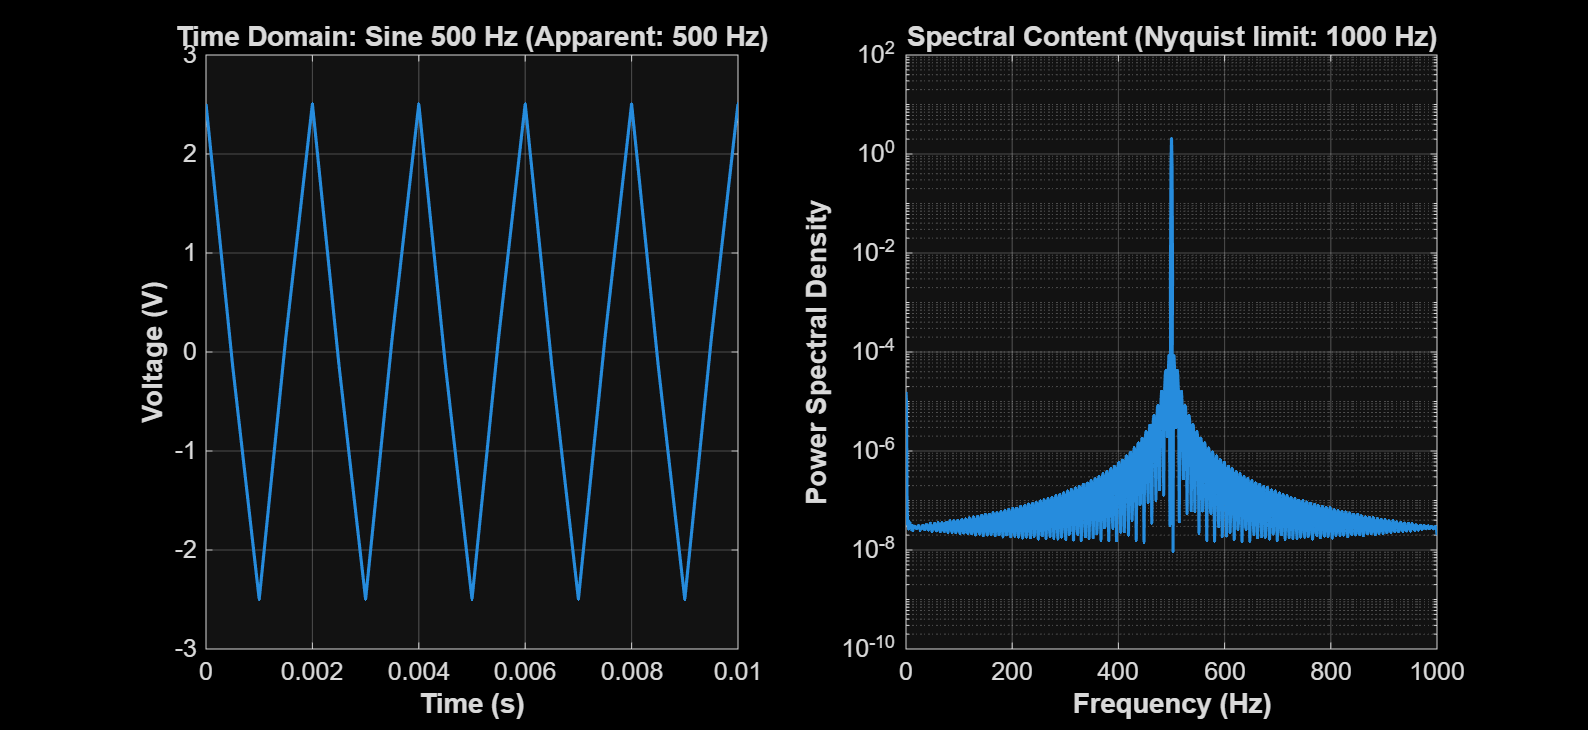
\includegraphics[width=\textwidth]{../pictures/Sine_500Hz_5.000Vpp_fs2000.png}
    \caption{\SI{500}{\hertz} Signal (Properly Sampled)}
  \end{subfigure}
  \hfill
  \begin{subfigure}{0.48\textwidth}
    \centering
    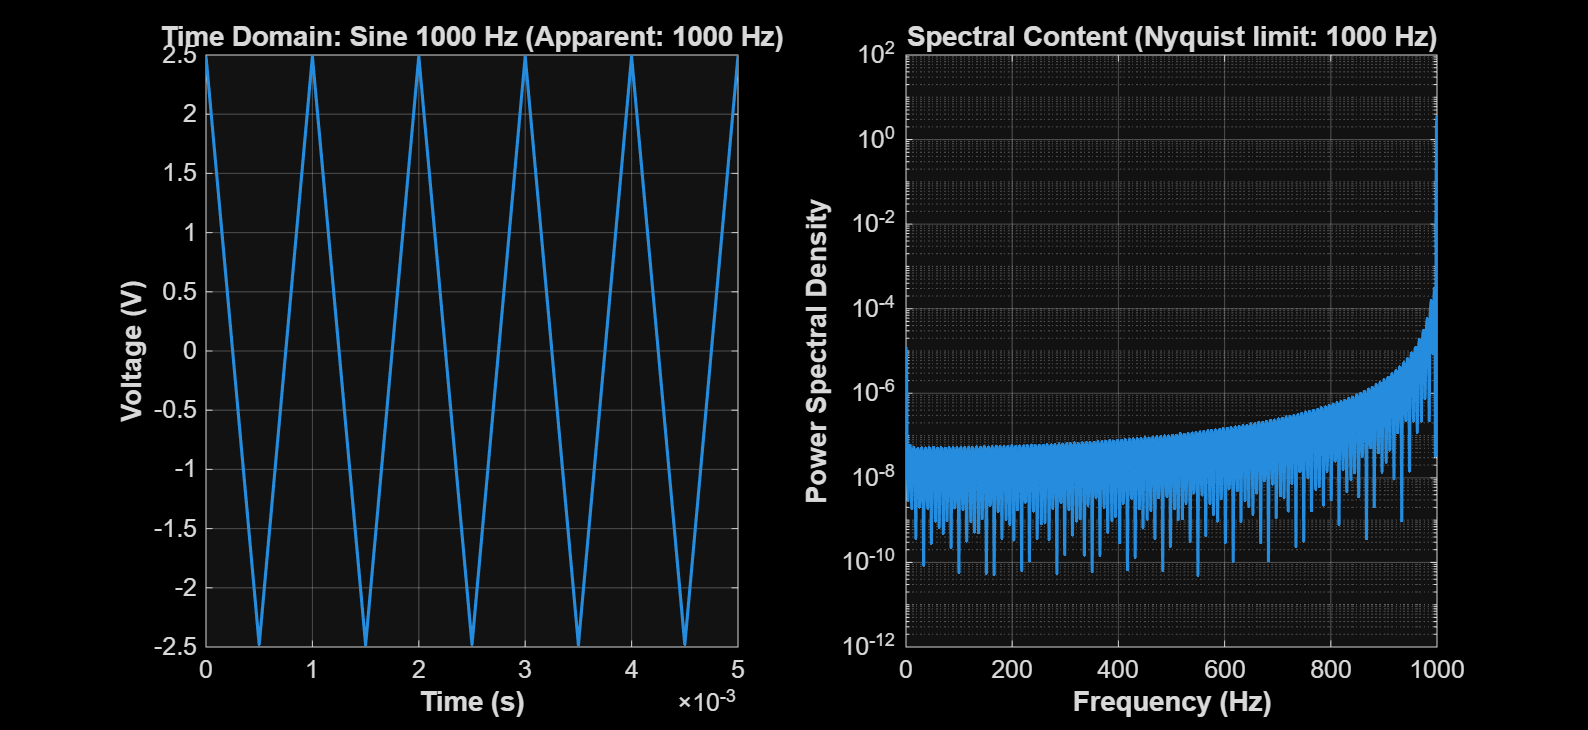
\includegraphics[width=\textwidth]{../pictures/Sine_1000Hz_5.000Vpp_fs2000.png}
    \caption{\SI{1000}{\hertz} Signal (At Nyquist Limit)}
  \end{subfigure}

  \vspace{0.5cm}

  \begin{subfigure}{0.48\textwidth}
    \centering
    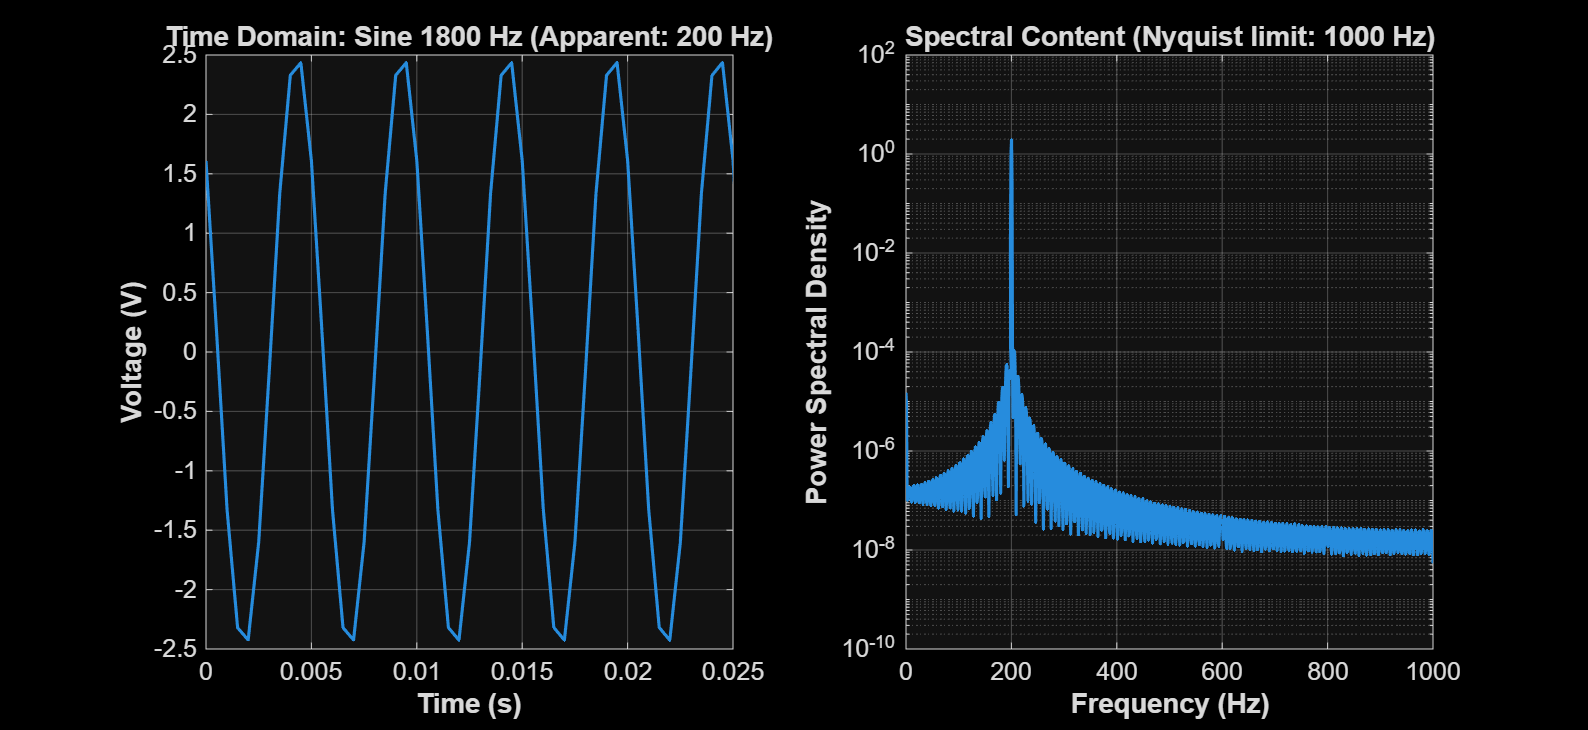
\includegraphics[width=\textwidth]{../pictures/Sine_1800Hz_5.000Vpp_fs2000.png}
    \caption{\SI{1800}{\hertz} Signal (Aliased to \SI{200}{\hertz})}
  \end{subfigure}
  \hfill
  \begin{subfigure}{0.48\textwidth}
    \centering
    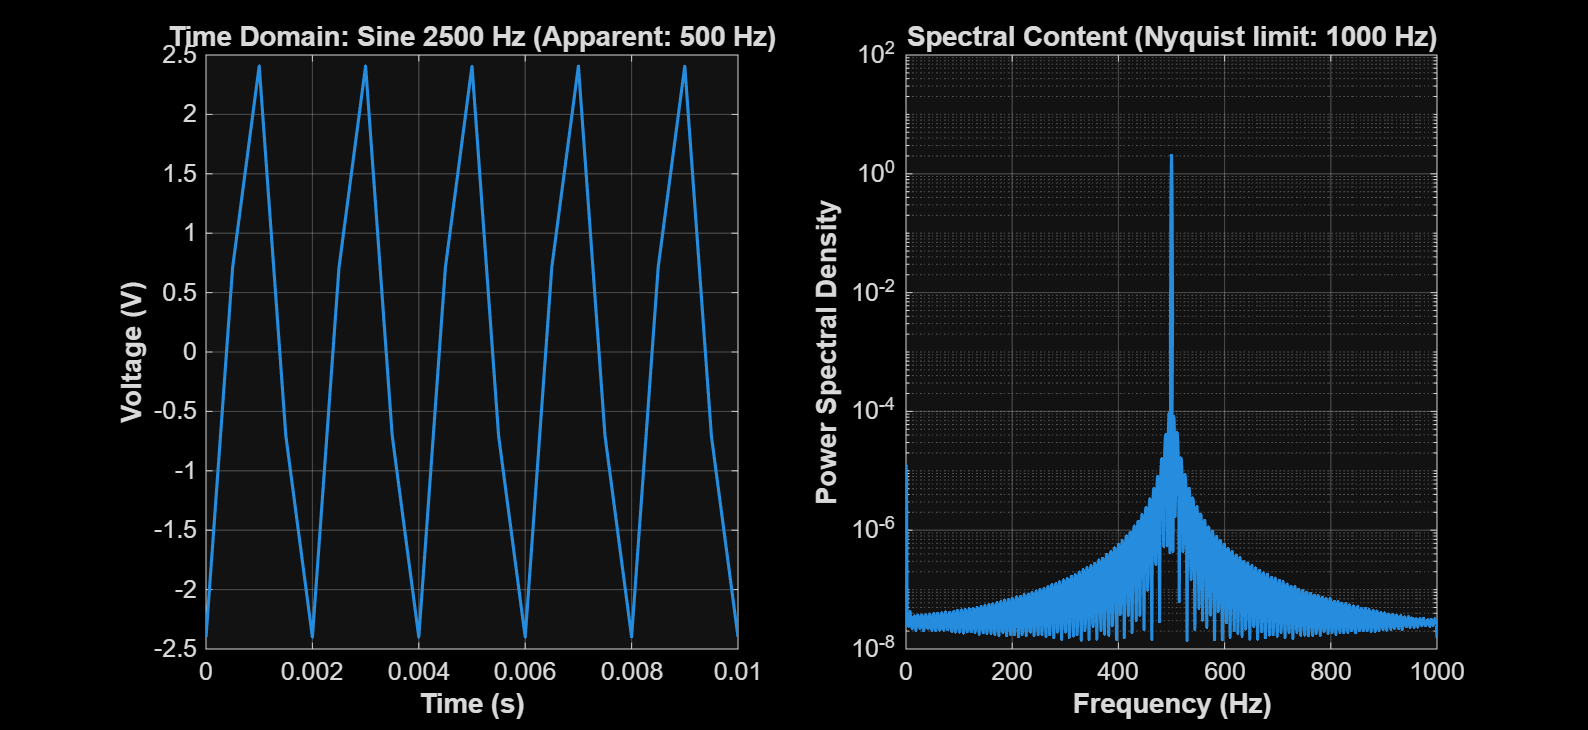
\includegraphics[width=\textwidth]{../pictures/Sine_2500Hz_5.000Vpp_fs2000.png}
    \caption{\SI{2500}{\hertz} Signal (Aliased to \SI{500}{\hertz})}
  \end{subfigure}
  \caption{Task 1: Selected Sine Wave Sweeps at $f_s = \SI{2000}{\hertz}$.}
\end{figure}

% ---------------------------------------------------------
% PART 2: HARDWARE RESOLUTION
% ---------------------------------------------------------
\newpage
\section*{Part 2: Limits of DAQ Hardware Resolution}

In this task, a \SI{100}{\hertz} sine wave was sampled at $f_s = \SI{10000}{\hertz}$. The amplitude was progressively decreased to observe the quantization limits of the 16-bit NI-6321 DAQ system operating across a $\pm\SI{10}{\volt}$ range.

\begin{figure}[H]
  \centering
  \begin{subfigure}{0.48\textwidth}
    \centering
    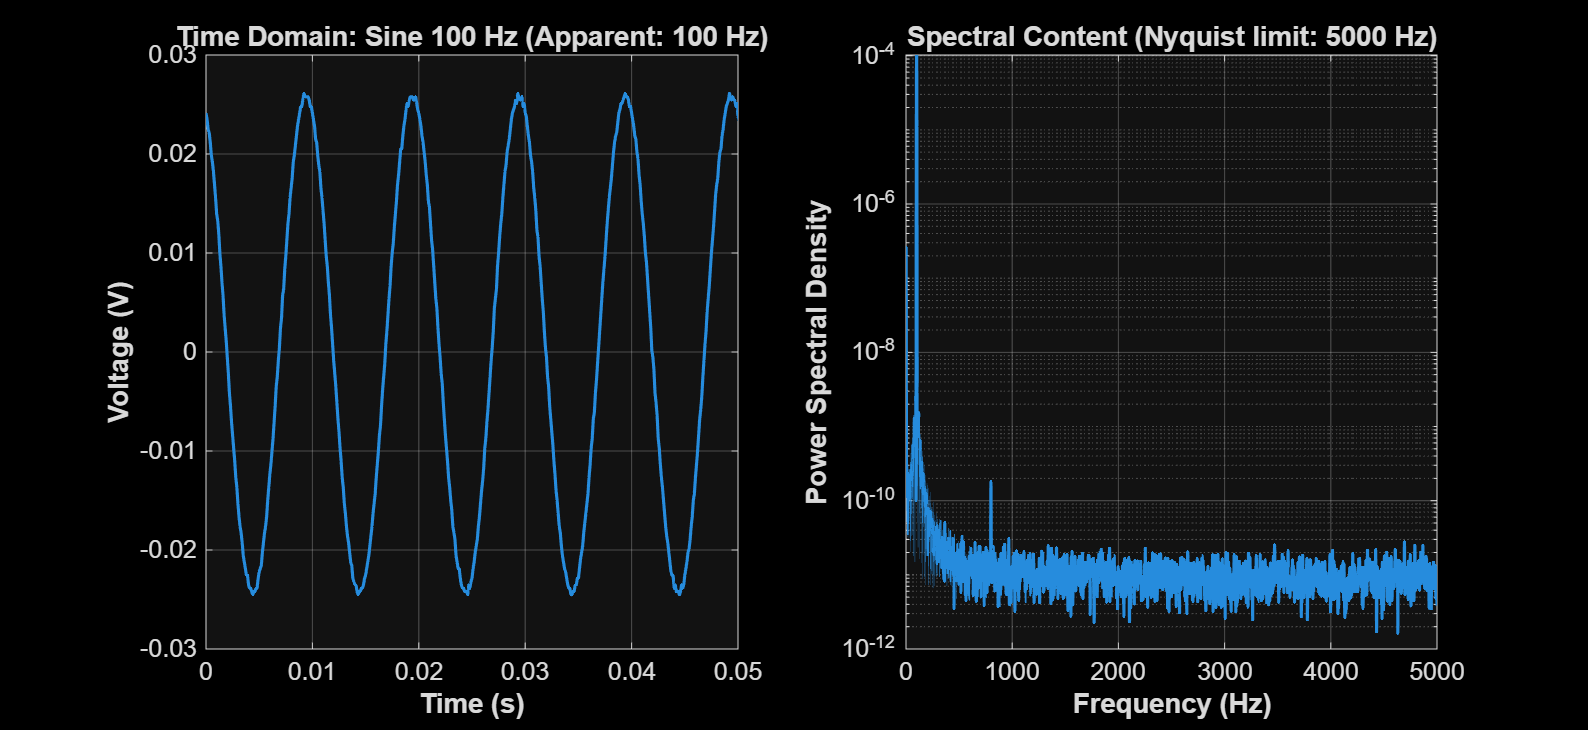
\includegraphics[width=\textwidth]{../pictures/Sine_100Hz_0.050Vpp_fs10000.png}
    \caption{\SI{50}{\milli\volt} Peak-to-Peak}
  \end{subfigure}
  \hfill
  \begin{subfigure}{0.48\textwidth}
    \centering
    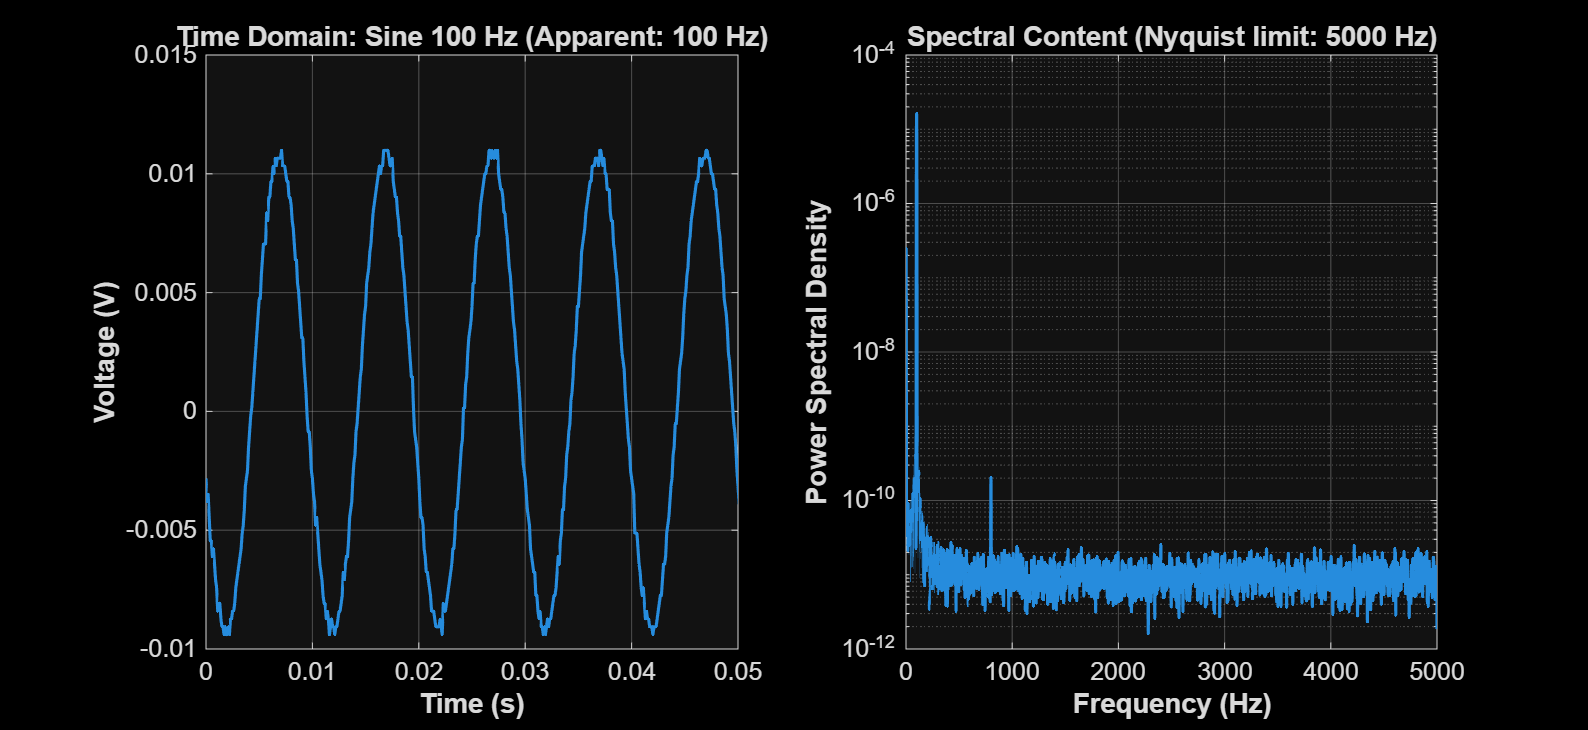
\includegraphics[width=\textwidth]{../pictures/Sine_100Hz_0.020Vpp_fs10000.png}
    \caption{\SI{20}{\milli\volt} Peak-to-Peak}
  \end{subfigure}

  \vspace{0.5cm}

  \begin{subfigure}{0.48\textwidth}
    \centering
    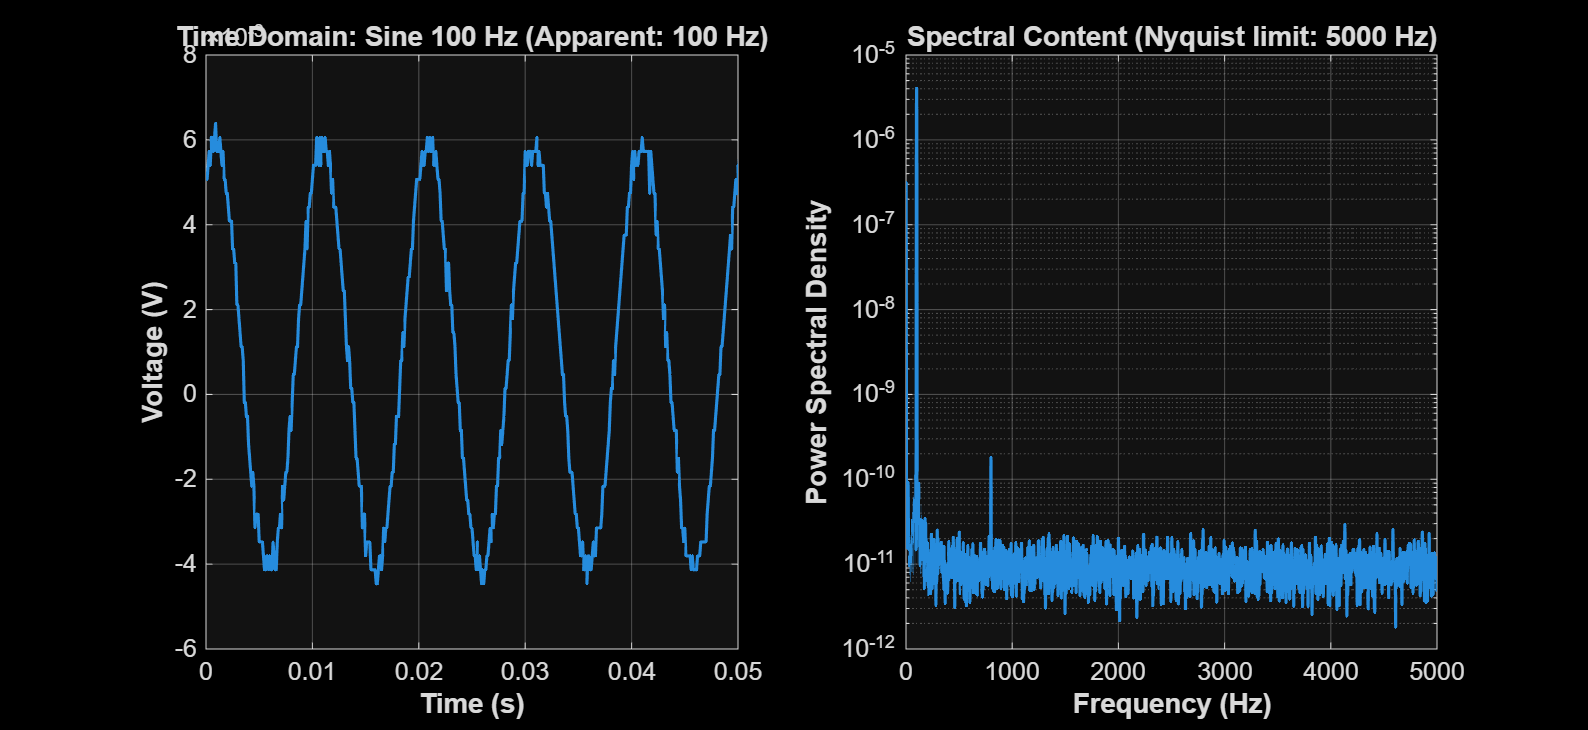
\includegraphics[width=\textwidth]{../pictures/Sine_100Hz_0.010Vpp_fs10000.png}
    \caption{\SI{10}{\milli\volt} Peak-to-Peak}
  \end{subfigure}
  \hfill
  \begin{subfigure}{0.48\textwidth}
    \centering
    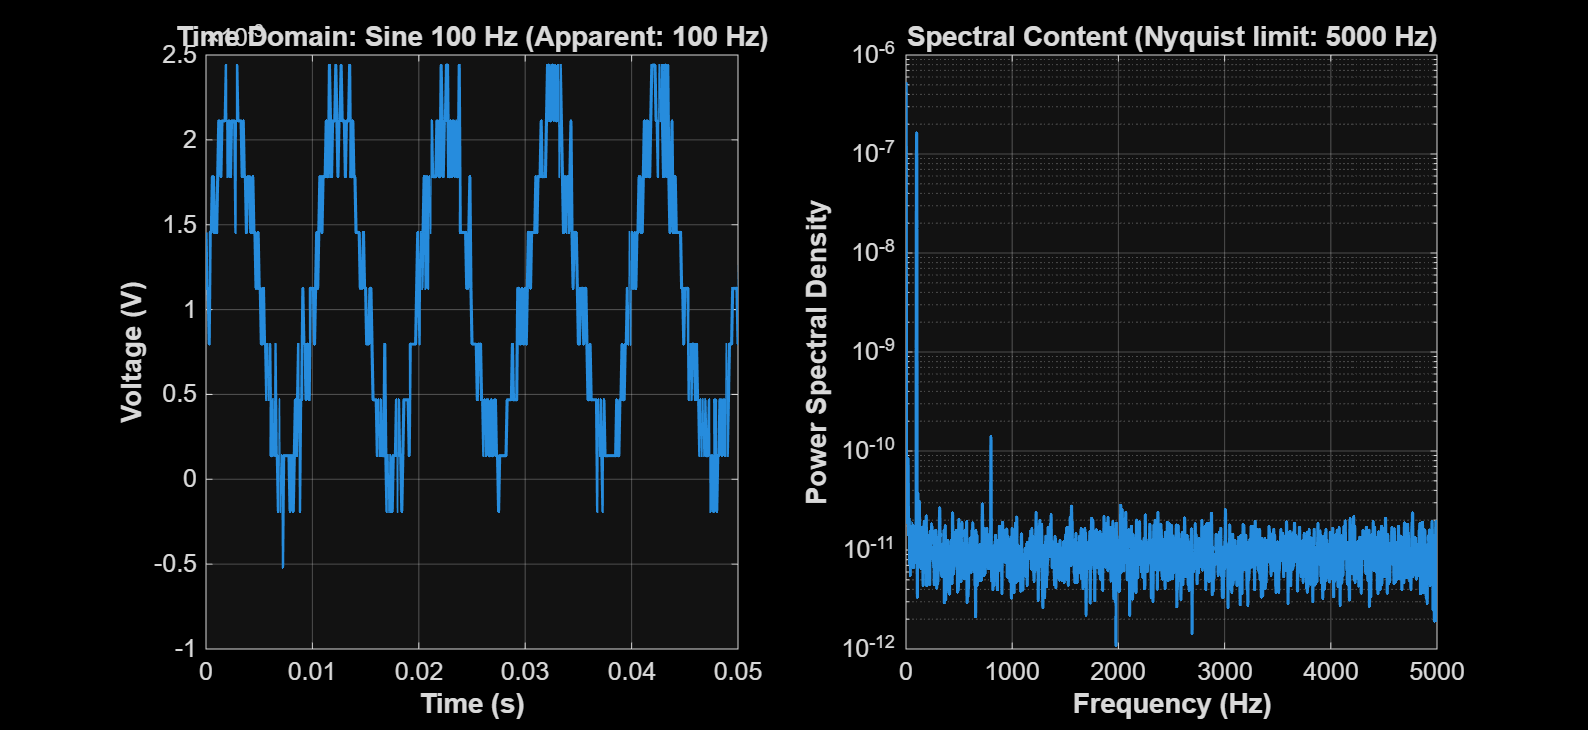
\includegraphics[width=\textwidth]{../pictures/Sine_100Hz_0.002Vpp_fs10000.png}
    \caption{\SI{2}{\milli\volt} Peak-to-Peak (Severe Quantization)}
  \end{subfigure}
  \caption{Task 2: Amplitude sweeps demonstrating DAQ resolution limits.}
\end{figure}

% ---------------------------------------------------------
% PART 3: NYQUIST LIMITS ON COMPLEX WAVES
% ---------------------------------------------------------
\newpage
\section*{Part 3: Undersampling Complex Waveforms (Sawtooth)}

In this task, a \SI{173}{\hertz} sawtooth wave (\SI{5}{\volt} peak-to-peak) was recorded at four different sampling rates to observe how the Nyquist limit truncates the higher-order harmonics required to form sharp waveform edges.

\begin{figure}[H]
  \centering
  \begin{subfigure}{0.48\textwidth}
    \centering
    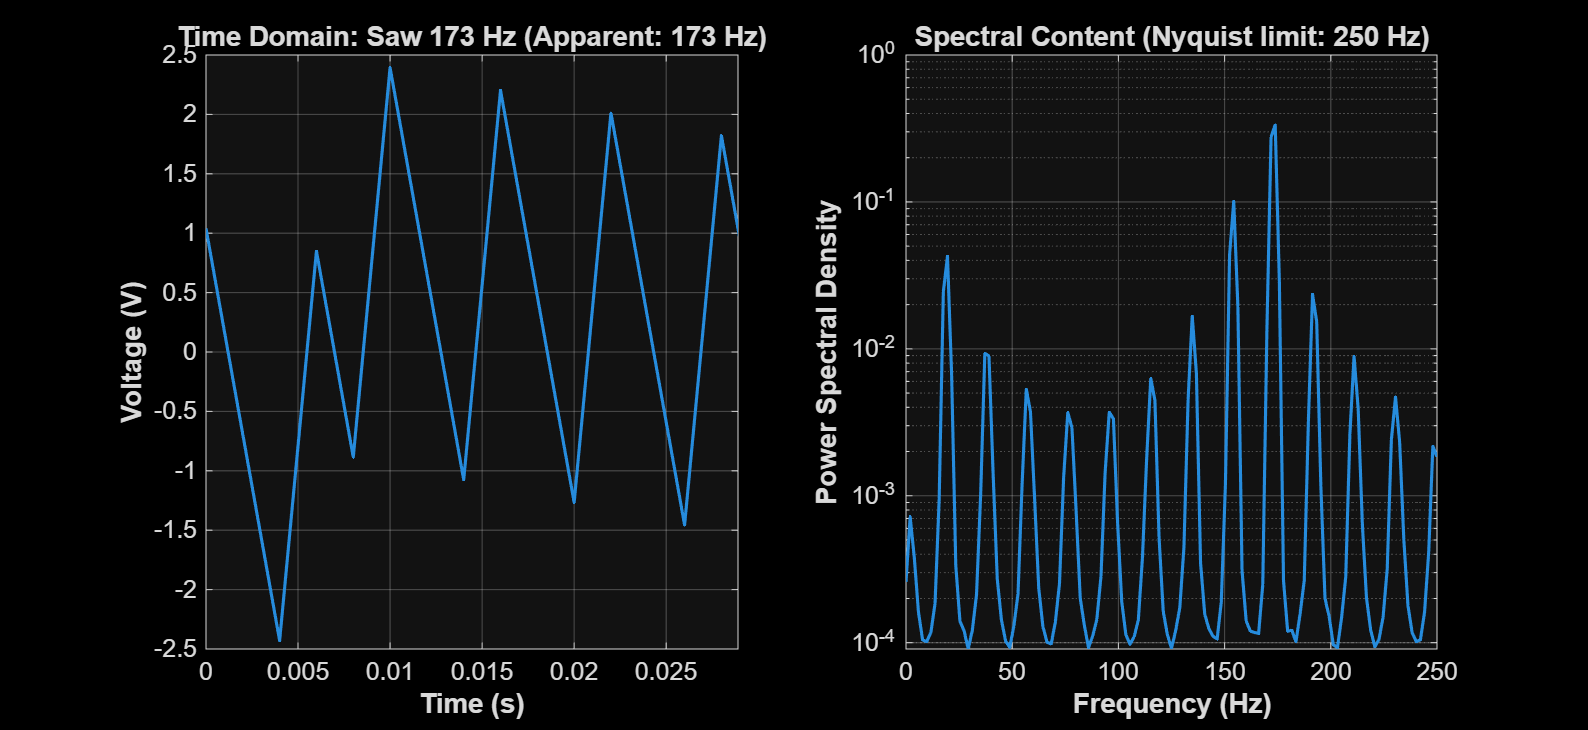
\includegraphics[width=\textwidth]{../pictures/Saw_173Hz_5.000Vpp_fs500.png}
    \caption{$f_s = \SI{500}{\hertz}$ (Nyquist = \SI{250}{\hertz})}
  \end{subfigure}
  \hfill
  \begin{subfigure}{0.48\textwidth}
    \centering
    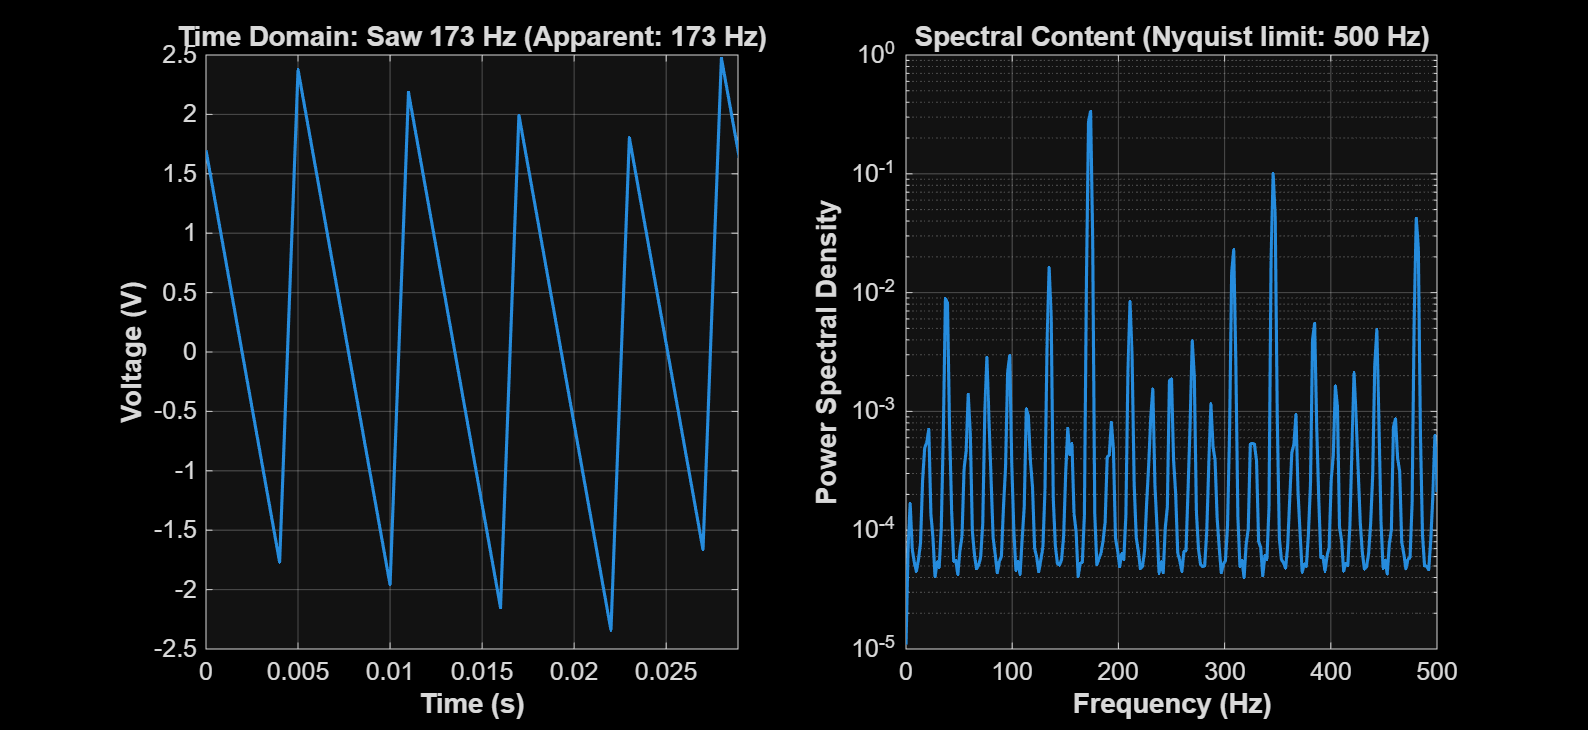
\includegraphics[width=\textwidth]{../pictures/Saw_173Hz_5.000Vpp_fs1000.png}
    \caption{$f_s = \SI{1000}{\hertz}$ (Nyquist = \SI{500}{\hertz})}
  \end{subfigure}

  \vspace{0.5cm}

  \begin{subfigure}{0.48\textwidth}
    \centering
    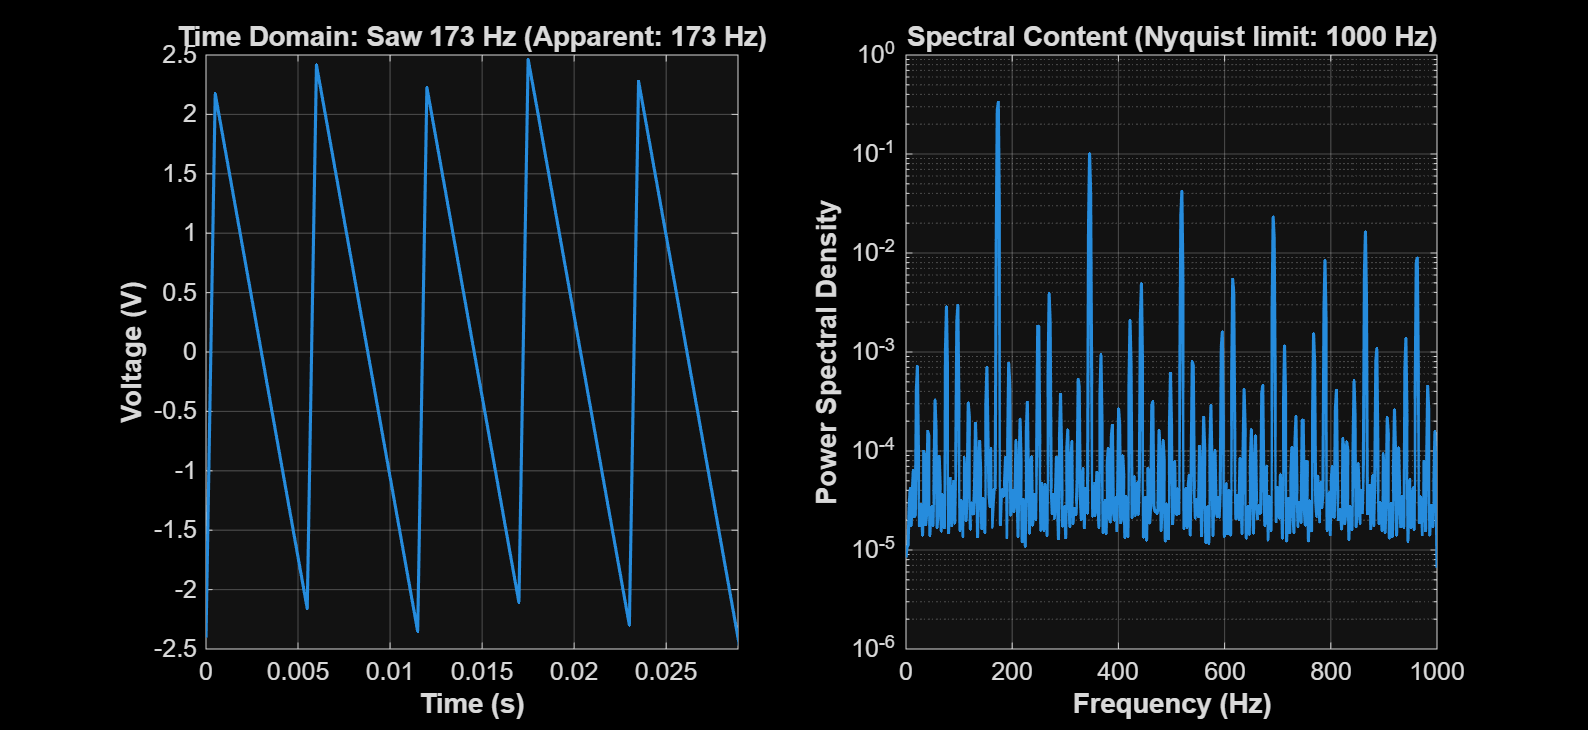
\includegraphics[width=\textwidth]{../pictures/Saw_173Hz_5.000Vpp_fs2000.png}
    \caption{$f_s = \SI{2000}{\hertz}$ (Nyquist = \SI{1000}{\hertz})}
  \end{subfigure}
  \hfill
  \begin{subfigure}{0.48\textwidth}
    \centering
    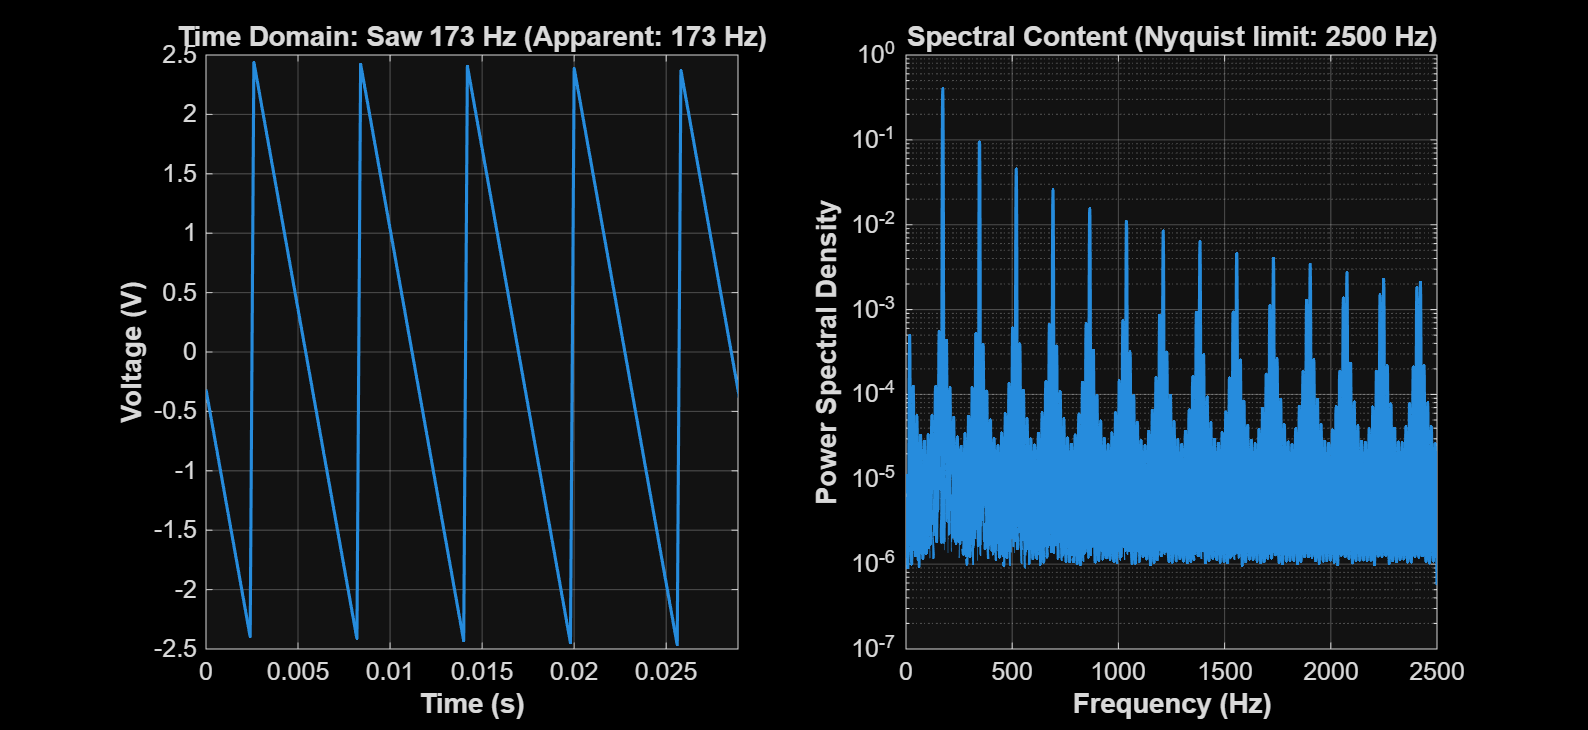
\includegraphics[width=\textwidth]{../pictures/Saw_173Hz_5.000Vpp_fs5000.png}
    \caption{$f_s = \SI{5000}{\hertz}$ (Nyquist = \SI{2500}{\hertz})}
  \end{subfigure}
  \caption{Task 3: Sawtooth wave at \SI{173}{\hertz} recorded across increasing sampling rates.}
\end{figure}

% ---------------------------------------------------------
% DISCUSSION
% ---------------------------------------------------------
\newpage
\section*{Discussion and Quantitative Analysis}

\textbf{1. Aliasing Behavior and Figure 7.3 Comparison (Task 1)} \\
When sampling at $f_s = \SI{2000}{\hertz}$, the theoretical Nyquist limit is exactly \SI{1000}{\hertz}. Any signal frequency exceeding this limit will fold back into the measurable range according to the absolute value equation $f_a = |f_{signal} - N \cdot f_s|$.

When mapping our 21 recorded alias frequencies against Figure 7.3 in the textbook, the empirical data perfectly traces the theoretical "folding" diagram:
\begin{itemize}
  \item \textbf{The Linear Rise:} From \SI{500}{\hertz} up to \SI{1000}{\hertz}, the signal is properly sampled ($f_{signal} < f_{Nyquist}$). The apparent frequency matches the input frequency precisely, representing the initial linear upward slope in Figure 7.3.
  \item \textbf{The First Fold:} At \textbf{\SI{1000}{\hertz}}, the signal sits exactly at the Nyquist peak. As the input sweeps past this limit (from \SI{1100}{\hertz} to \SI{2000}{\hertz}), the apparent frequency "folds" backward, decreasing linearly down to a trough of \SI{0}{\hertz} at $f_s = \SI{2000}{\hertz}$. Our data cleanly follows this downward slope (e.g., \SI{1800}{\hertz} aliases to exactly \SI{200}{\hertz}).
  \item \textbf{The Second Fold:} As the signal exceeds the sampling frequency itself (\SI{2100}{\hertz} to \SI{2500}{\hertz}), the apparent frequency reflects off the \SI{0}{\hertz} trough and begins rising linearly again. This mirrors the second upward slope in Figure 7.3, confirmed by our \SI{2500}{\hertz} input aliasing exactly back to \SI{500}{\hertz}.
\end{itemize}

\textbf{2. DAQ Hardware Resolution and Quantization Error (Task 2)} \\
The NI-6321 DAQ is a 16-bit device operating on a $\pm\SI{10}{\volt}$ scale. This yields a total span of \SI{20}{\volt}. The minimum measurable voltage step (quantization interval, $Q$) is:
\[ Q = \frac{E_{FSR}}{2^M} = \frac{20\text{ V}}{2^{16}} = \frac{20\text{ V}}{65,536} \approx \mathbf{0.305 \text{ mV}} \]
For the \SI{50}{\milli\volt} signal, the waveform covers approximately 164 discrete steps, producing a relatively smooth sine wave. However, the \textbf{\SI{2}{\milli\volt} peak-to-peak} signal spans an extremely narrow range. Quantitatively, the entire signal is forced to fit within just $\frac{2 \text{ mV}}{0.305 \text{ mV/step}} \approx \mathbf{6.5 \text{ steps}}$.

As a result, the time-domain plot of the \SI{2}{\milli\volt} signal transforms into a blocky, ``stair-step'' function. In the spectral plot, this severe quantization error manifests as broadband noise and spurious high-frequency harmonics. Because a square, stair-step shape requires many higher-order frequencies to construct mathematically, the spectral energy is scattered far beyond the fundamental \SI{100}{\hertz} peak. This emphatically proves the necessity of analog signal conditioning—small signals must be amplified to span the DAQ's full resolution range before digitization to preserve fidelity.

\textbf{3. Nyquist Limits on Complex Waveforms (Task 3)} \\
Unlike a sine wave, a \SI{173}{\hertz} sawtooth wave is a complex signal constructed from an infinite sum of both even and odd harmonics. The sharp, vertical drop-off of the sawtooth requires extreme high-frequency content to reconstruct mathematically.
\begin{itemize}
  \item At $f_s = \textbf{\SI{500}{\hertz}}$, the Nyquist limit is \SI{250}{\hertz}. This acts as a severe digital low-pass filter, chopping off every harmonic above the fundamental \SI{173}{\hertz} tone. Consequently, the resulting plot looks like a distorted sine wave, entirely stripped of its sawtooth characteristics.
  \item At $f_s = \textbf{\SI{1000}{\hertz}}$ and \textbf{\SI{2000}{\hertz}}, we begin to capture the 2nd through 5th harmonics. The wave begins to skew and lean to the right, slowly building the sawtooth profile.
  \item At $f_s = \textbf{\SI{5000}{\hertz}}$, the Nyquist limit is \SI{2500}{\hertz}. This successfully captures up to the 14th harmonic ($173 \times 14 = 2422 \text{ Hz}$). This abundance of high-frequency energy allows the sudden, sharp voltage drop to be accurately drawn.
\end{itemize}

% ---------------------------------------------------------
% APPENDIX
% ---------------------------------------------------------
\newpage
\appendix
\section*{Appendix: MATLAB Code}

\subsection*{Lab5\_RecordData.m}
\lstinputlisting[language=Matlab]{../Lab5_RecordData.m}

\subsection*{Lab5\_Analysis.m}
\lstinputlisting[language=Matlab]{../Lab5_Analysis.m}

\end{document}
